% put environments that should be ignored by texcount here, e.g., here lstlisting for code

%TC:envir lstlisting [] ignore

%for reference to this section
\section{Introduction}
\label{section:Introduction}

% Vielleicht vorher noch eine Einführung (am besten mit Referenzen) warum mehr als nur die kürzeste Route relevant sein kann.

The selection of a route to get from one spot to another is a fundamental aspect of pedestrian behavior. \autocite[]{Bierlaire2009} The vast majority of simulation tools employ straightforward route selection models that consider only the shortest walking distance or walking time between a passenger's origin and destination. \autocite[]{Daamen2005} But different surrounding aspects and impacts have an influence on the route choice of pedestrians and have been discussed and analyzed in multiple previous studies. The impact of attractiveness of a street to the route choice in a shopping context was discussed by \autocite[]{Kurose2001}. \autocite[]{Borst2008} described the relationship between perceived attractiveness of streets and the physical street characteristics. The importance of distance, while the level of congestion, safety, or visual attractions appear to be secondary was found out by \autocite[]{Morrall1985} analyzing and evaluation factors affecting the route choice. Convenience, attractiveness, simplicity, availability of facilities and availability of landmarks have been the main attributes taken into account by \autocite[]{Millonig2007} as influences to the quality of a specific route. Following this previous research on factors affecting passenger route choice this paper aims to use pedestrian traffic as its main factor influencing the route to indicate a correlation between the pedestrian traffic and route satisfaction.



To indicate how this factor is valued a correlation between the pedestrian traffic and route satisfaction will be used.





Also, the way these factors influence route choice behavior needs to be determined to indicate how each factor is valued \autocite[]{Daamen2005}




This paper aims to get a correlation between pedestrian traffic and route satisfaction.


get a correlation between 
Given an open GPS Trajectories Dataset from the OpenStreetMap project, the research was conducted on the historical walking data in the City of Salzburg in Austria. 


Due to the city's historical growth, footpaths, pedestrian areas, and private and public transport roads are limited to change and urban development (SOURCE). 

\autocite[]{Netsch2021}

Historical traffic pattern mining and analysis for traffic forecasting and improving traffic flow is broadly used and common to vehicle traffic management. Multiple studies focus on collecting data, analyzing patterns, and forecasting traffic flow for vehicle traffic. 

Is it possible to increase satisfaction by recommending alternative, less populated routes to tourist attractions using pedestrian path model techniques?

The research is going to be structured into a background section, related work, a section describing the methods used, a system overview, implementation details and an evaluation section.

\section{Background}
Walking and choosing routes in the city of Salzburg is due to the big tourism never a simple task. Many shortest routes are going through points of interests and showplaces used by tourist agencies for their route planning making the daily commuting hard for locals. The cities street network due to its historical growth also has not the biggest number of alternative routes for walking to offer. That results in packed walking paths during the entire year.

Further, the covid pandemic has brought a factor of distancing and trying to avoid big crowds 


Lorem ipsum dolor sit amet, consectetur adipiscing elit. 

\section{Related Work}
Introduce why this specific related work is important for your own work. Which areas do you cover and why? What do you take as inspiration and what do you do differently/improve upon? 

\autocite[]{Sevtsuk2021}

\autocite[]{Delling2012}
\autocite[]{Hashemi2017}
\autocite[]{Qiu2015}
\autocite[]{Hendawi2019}
\autocite[]{Huber2016}

\autocite[]{Zhang2012}

\section{Methods}

This section discusses the methods and frameworks that have been used to calculate and propose the new route further used in this research. 

Proposing the alternative route will be done by using the influence of historical pedestrian traffic to calculate a route with fewer interactions for the traveler to get to the same goal. This will be done by analyzing historical GPS trajectories and using a customized routing engine to propose a route then evaluated through a trail run. 

In order to achieve the objective of customizing a routing engine several processing and classifying steps are needed in advance as most GPS traces are stored in plain text formats without any associated metadata, such as mode of transportation, distance, or speed. And such metadata not only simplifies the analysis, mining, and visualization of vast quantities of GPS traces, but also prepares the way for automatic GPS trace applications. \autocite[]{Hashemi2017}

After that processing and classification the trajectories have to be assigned to the street network to know how many routes have been taken on which street. This is necessary to be able to influence the routing engine with the traffic patterns as the streets will be virtually made longer by the routes counted on each path.

The methods used are the following: \textit{Pre-Processing} to convert and cleanup, \textit{Classification} to separate the traces into modes of transportation, \textit{Map-Matching} to align the traces on the paths and streets taken, \textit{Reverse Geo-coding} to find out through which paths and streets the traces are going, \textit{Map adaptations} to adapt the street network to the pedestrian traffic patterns and \textit{Customized Routing} to suggest a new route based on the influence of the traces.

\subsection{Pre-Processing}

In the Pre-Processing Phase the trajectories are going to be prepared for the classification. This will happen mainly through the conversion to a JSON format and an outlier removal to cleanup the dataset before further categorization. After that the traces will be programmatically and validated, meaning they will tested for their integrity and then be projected onto a visual map for inspection.

Convert & Cleanup Traces.
Validate Traces.

Classification.

That is the reason for adding a pre-processing phase to prepare the trajectories for classification and then do so for them to be further used. Pre-processing mainly is the conversion to a JSON format and an outlier removal to cleanup the dataset before further categorization. 


\subsection{Classification}

As the dataset will not have any metadata differentiating the routes and the scope of the research only need to take walking trips in consideration all given routes need to be classified. The main classification factor is the mode of transportation which is in the researches case is walking. 

The classification will be carried out in three steps to sort out as many non-walking trips as possible before handing the traces over to the map-matching phase. These steps are based on two principles. Firstly finding keywords in the traces description signaling that the mode of transportation was either by car, bus or bike. And secondly using average speed calculations, both on the full route and on segmented parts of the route. The segmentation will be done using fixed frames to signal if parts of the route were taken with modes of transportation other than walking. This was done on the basis of the pre-processing and classification process used by \autocite[]{Qiu2015}. The decision not implementing the stop detection algorithm proposed in the same research was made as routes that have segments of using other modes of transportation were not split-up but not used for further research at all. Separating all route segments, classifying and then validating them would have gone beyond the scope of this study.

Further the use of Map-Matching and using the customized router with routing profiles only keeping walk paths in consideration for the route makes the lack of a further classification to have less of an impact to the route proposal.

The average walking speed was selected doing research in the field of sports and walking behaviours. (Source)

and is based on keyword  average speed calculations


a classification of all given routes has to be  

To differentiate if a walk 

The classification used is based on average speed calculations to sort out as many non-walking trips as possible before handing the traces over to the map-matching phase. As just using the whole traces average speed is not able to 

To get the metadata needed for further processing the classification phase is p 


be able to classify the trajectories to then be used. 

To build the historical walking patterns 


\subsection{Map-Matching}

To use the historical walking trips the trajectories have to be connected to the streets and paths taken to build walking patterns. To be able to do this a map-matching algorithm will be used to combine positioning data with spatial road network data to identify the correct link on which the data was collected. \autocite[]{Quddus2007} In other words, locational data must be reconciled with map or network data, and map-matching algorithms are utilized to accomplish this task. \autocite[]{Greenfeld2002} Further if accurate spatial road network data are available, map-matching not only enables the actual location of the vehicle to be detected, but it also enhances the positioning accuracy. \autocite[]{Ochieng2003}


Map-matching algorithms use inputs generated from positioning technologies and supplement this with data from a high resolution spatial road network map to provide an enhanced positioning output. 

The general purpose of a map-matching algorithm is to identify the correct road segment on which the vehicle is travelling and to determine the vehicle location on that segment (Greenfeld, 2002; Quddus et al., 2003). Map-matching not only enables the physical location of the vehicle to be identified but also improves the positioning accuracy if good spatial road network data are available (Ochieng et al., 2004). This means that the determination of a vehicle location on a particular road identified by a map-match- ing algorithm depends to a large extent on the quality of the spatial road map used with the algorithm. A poor quality road map could lead to a large error in map-matched solutions.




Map-matching algorithms integrate positioning data with spatial road network data (roadway centrelines) to identify the correct link on which a vehicle is travelling and to determine the location of a vehicle on a link. A map-matching algorithm could be used as a key component to improve the performance of systems that support the navigation function of intelligent transport systems (ITS) \autocite[]{Quddus2007}


\subsection{Reverse Geo-coding}

As now the trajectories are properly matched to the paths they have been taken on to create the historical patterns the streets they are laying on have to be identified. This is done by using a reverse Geo-coding process. The reverse Geo-coding process is the opposite of the Geo-coding process. Individuals, research groups, and organizations of all sizes across the globe, ranging from not-for-profit and commercial entities to local, state, and national-level government agencies, are frequently required to perform geocoding for a variety of extremely important and mission-critical tasks. Across the globe, these geocoding services are in high demand. \autocite[]{Goldberg2013} Commercially it is used, for example,  in the Google Maps tool to find locations based on their name. So Geo-coding is the process of connecting an address record with a point on a map. \autocite[]{Ratcliffe2001} That means reverse Geo-coding is the extraction of textual information, that is readable by humans, such as a name or an address, from geographic coordinates (latitude, longitude). \autocite[]{Kounadi2013}

Services that handle a coordinate in a manner analogous to that of the Geo-coding operation are able to do methodically what is known as reverse Geo-coding.
For example, when a GPS coordinate is provided, the street address is interpolated from a range that is assigned to the road segment in a reference dataset to which the point is closest. This ensures that the street address is as accurate as possible. 

Each map-matched GPS point is going to be fed to the reverse Geo-coding algorithm to get each exact location information. The location information will be filtered on only using streets and paths as building information is not influential for further analyzes. Having each location data on a route, to avoid counting a street multiple times and distorting the outcome, consecutive street and path data information will be summarized till a new way will be taken.   

\subsection{Map Adaptions}

Having the count of trajectories going through the street and path network of the analyzed map section, the map has to be adapted so the routing engine is able to use the factor of the historical pedestrian traffic patterns to propose a new route. Therefore the map data used to configure the routing algorithm will be extended with the data collected from the reverse Geo-coding process. This will be done using a Map Editor Software.

\subsection{Routing}





% Struggles from Hashemi to relate here too.
% Cite:
%
%However, GPS traces are stored in plain text formats with no attached metadata such as, transpor- tation mode, length, or speed. This not only makes managing large volumes of GPS traces inefficient but also restricts the scale and scope of algorithms for human mobility pattern detection. Open Street Map (OSM), founded in UK in 2004 with more than 1 million registered users (Wood, 2013), is the most prominent volunteered geographic information devoted to providing a free map of the world empha- sizing the road networks. Road networks are built upon GPS traces uploaded by registered users and can be edited or updated manually at any time. A description can be associated to a GPS trace while being uploaded but there are no additional required metadata or restrictions (https://www.open- streetmap.org/traces; OpenStreetMap, n.d.). This means the transportation mode of the GPS trace (e.g. walking, motoring, or boating) cannot be known in the database which in turn limits the data- base’s applications. Besides, they do not store additional metadata, such as average speed or total length of the GPS trace which can be automatically calculated. Such metadata not only facilitates analyzing, mining, and visualizing large volumes of GPS traces, but also paves the path for automatic applications of GPS traces. Examples of such applications are automatic road and pedestrian network construction (Hashemi, 2017b), recognizing POIs (Bhattacharya, Kulik, & Bailey, 2015), developing intelligent location-based services (Liu & Karimi, 2006), detecting individual (Song et al., 2010), or collective (Becker et al., 2013; Harder, Nes, Jensen, Reinau, & Weber, 2012) mobility patterns, and real-time event detection which is of great value to municipalities, police, and fire departments.
%
%



To begin analysing and classifying the GPS traces several filtering related processes lowering the effects of noice and to identify higher level semantic information to reduce the size of analysed data. 

To reduce the size of analysed data several filtering related processes to lower the effects of noice and to identify higher level semantic information 


Most of the existing work [17, 23], that analyse behaviour
patterns of individuals from their GPS traces will begin from several filtering related processes in order to reduce the size of analysed data, to lower the effects of noise, and finally to identify higher level semantic information as outputs. 


In order to achieve these objectives, we explored existing methods in different levels and investigate a computation framework for semantic trajectory analysis, which is based on the model proposed in [17]. As a tiered computing framework, it accepts users’ outdoor GPS trajectories data as input and facilitates the discovery of their higher-level behaviour patterns, which in this particular work will be the frequent activity patterns of an individual.
A.



\section{System Overview}

Provide a high level overview of your system, approach, etc. 
Describe features, user interfaces, provide screenshots.
What does a user do with your application/system/interaction method?

In order to build a system to propose an alternative route to answer this researches question systems, software and data sources are needed to do so. As the scope of this study lies on finding out about an increase or decrease of the proposed route satisfaction, and the route proposal is the tool to answer that question, the methods as described will rely mainly on already existing solutions adapted to the research and not propose new ways of the methods selected to do so. 

To be able to build those historical pedestrian travel patterns to propose a new route a map, map data, mapping tools & algorithms and a route engine needed to be found and selected according to the researches terms and methods. For that an in depth research of services and solutions was carried out using keywords like "Map software", "Map tools" and "Map router" using online search engines.

Outcome of that research were solutions both commercially and open-source.

Commercial applications and tools like Google Maps \footnote{\url{https://developers.google.com/maps}}, Mapbox \footnote{\url{https://www.mapbox.com/}} or Here \footnote{\url{https://developer.here.com/}} offer a lot of services to conduct operations on their provided map instances yet the free quotas and the customization for the mapping tools and routing are very limited. 

Due to that limitation of customization, which was one of the main terms for the method and tools selection, open-source alternatives that enable an adaption had to be taken in consideration. And the biggest and most popular open-source project, the OpenStreetMap (OSM) \footnote{\url{https://www.openstreetmap.org/}} and its ecosystem of mapping tools, routing engines and community fit ideally to be used further.

The OpenStreetMap project has seen a dramatic growth in the volume of provided spatial data during the previous five years. A large number of places already have high-quality data that rivals or exceeds commercial map data. \autocite[]{luxen-vetter-2011}

That increase in interest in OSM has also resulted in the creation of many tools and methodologies to assess its quality, to enhance OSM Data by means of algorithms tailored to specific object types, such as addresses for Geo-coding or artificial neural networks to detect the absence of metropolitan areas. OSM's crowd sourced Geo-data is now being used in a wide range of practical and scientific applications in a variety of fields, demonstrating the utility of the crowd sourced Geo-data in OSM following these and many other enhancements. \autocite[]{JokarArsanjani2015}




%figure* stretches figure over both columns
\begin{figure*}[!ht]
  \centering
  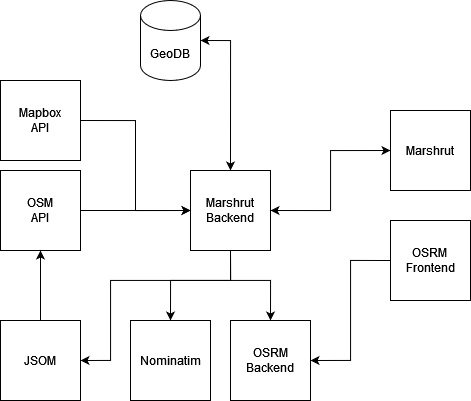
\includegraphics[width=0.5\textwidth]{images/SystemOverview.png}
  \caption{
  System Overview.
  }
  %for reference to this figure
  \label{figure:SystemOverview}
\end{figure*}


Given crowdedness as the main factor in calculating a new route, the crowdedness has to be measured to add traffic as a parameter to that route calculation. This will be achieved creating historical traffic patterns. To create such historical pedestrian traffic/walking patterns, a solid Data-set is needed so the routing engine can be configured to be adapted to the influence of the walking patterns. 

% To be able to propose a new route a map, map data, mapping tools and a route engine needed to be selected. 

% Commercial applications and tools like Google Maps, Mapbox or Placeholder offer a lot of services to conduct operations on their maps yet the customization for the mapping tools and routing are very limited. 

% Therefore open-source alternatives that allow and enable adaptions had to be taken in consideration. And the biggest and most popular open-source project, the OpenStreetMap (OSM) project and its ecosystem of mapping tools, routing engines and community 

% As the main factor of the research is the crowdedness of given pedestrian routes
% a way of measuring and adding traffic as a parameter to calculate new routes 
% an alternative route proposal a way of proposing that alternative is needed. The main factor traffic


To create the historical pedestrian traffic/walking patterns, a solid Data-set is needed so the routing engine can be configured to be adapted to the influence of the walking patterns. 

Searching for a Data-set that is viable for further analysis was not an easy task. There is no publicly available data from the city itself. Also, local research institutions contacted during the research period have no such data available. Therefore the OSM Project and its Database of public traces came in handy. Their collection is publicly accessible to be extracted, verified, classified, and then used to create a historical pedestrian traffic pattern for the part of the city that was used to create the alternative route.

Map Application



% \subsection{Map / Map Data}

\subsection{OpenStreetMap}

The OpenStreetMap is a free, editable map of the whole world that is being built by volunteers largely from scratch and released with an open-content license. 
\autocite[]{wiki:about}

The project was established in 2004 and has since become the Internet's most well-known example of Volunteered Geographic Information (VGI). \autocite[]{JokarArsanjani2015} 

The OSM mission statement came out of this simple concept, which was to produce a free, editable map of the world through collaboration. Instead of focusing on outputs in the form of cartographic products and maps, OSM's core is a geographical database including geographic data and information from around the world. \autocite[]{Antoniou2017}

It has a number of 8.805.780 users that contributed to 7.835.601.984 GPS locations making up 877.995.015 streets, paths and ways with 10.104.639 relations to each other and 11.771.986.020 GPS Points in GPS Traces. This makes it the largest community contributed and crowd sourced geographic information project in the world. (Source)


\subsection{OpenStreetMap Data}

The OpenStreetMap Project as described is a Geo-data Database. To work with that Database the structure and schema used to store the data had to be analyzed to understand its purpose and meaning. As a Geo-data provider, OSM describes all physical, natural, and human-made objects in a landscape that can be mapped as features. Features for example are Pavements, Statues, Churches, Streets or Bus Lines. To represent the features, OSM uses Elements attached with Tags. Elements are the basic components of the projects conceptual data model of the physical world.

There are three types of elements:

\begin{enumerate}
    \item Nodes
    
    A node is a point on the earth's surface that is identified by its latitude and longitude. Each node includes a unique identifier and a pair of coordinates. 
    
    \item Ways
    
    A way is an ordered list of two to two thousand nodes that defines a polyline. Typically, a way is a linear land feature (such as a road, wall, or river).
    
    \item Relations
    
    A relation is a multi-purpose data structure that documents a relationship between two or more data elements (nodes, ways, and/or other relations).
    
\end{enumerate}

Each of the aforementioned items can have one or more associated tags. Tags are key and value pairs which describe the meaning of a particular element. 

As a result, the key provides a description of a subject, category, or type of feature. It is possible to qualify keys with prefixes, infixes, or suffixes in order to define super- or sub-categories, as well as name-space. The majority of name-spaces have both a language specification and a date name-space specification for the name keys they offer. 



The key specifies a feature, and the value tells you what that feature is.
Free-form text, a single value from a set, numerous values from an enumeration, or a numeric value, such as a distance, are the most common types of values.
Although the key is self-explanatory, the tag value is still required. 





%Therefore, the key describes a subject, category, or type of feature. Keys can be qualified with prefixes, infixes, or suffixes to form super- or sub-categories, as well as namespace. For name keys, common namespaces include a language specification and a date namespace specification.

% OSM is principally a collection of geodata, meaning it is not the map itself but more the information on top of a visual map, 

% As OSM is a collection of map data 

% Elements are the basic components of OpenStreetMap's conceptual data model of the physical world. Elements are of three types:

%     nodes (defining points in space),
%     ways (defining linear features and area boundaries), and
%     relations (which are sometimes used to explain how other elements work together).



\subsection{OpenStreetMap Editing API}

The OSM Editing API is a collection of APIs based on RESTful API principles. There are API calls to create, read, update, and delete the three fundamental elements that makeup OpenStreetMap's map data. They each return or expect the data for the elements in an XML format.
\autocite[]{wiki:api}

The Data-points are returned using GPX (GPS Exchange Format) a XML data format for GPS data \footnote{\url{https://www.topografix.com/GPX/1/1/#type_trksegType}}. Important to mention is that in violation of the GPX standard, for privacy reasons, all waypoints of non-trackable traces are randomized and delivered as one track segment. 

GPX (the GPS Exchange Format) is a light-weight XML data format for the interchange of GPS data (waypoints, routes, and tracks) between applications and Web services on the Internet. 

Important to mention is that This happens in violation of the GPX standard. 

To further work with the data points 



% \subsection{Map Tools}

\subsection{Java OpenStreetMap Editor}

OSM is an openly accessible spatial database which any contributor can supply geodata to and whose existing data any contributor can also edit. It is therefore very important that software tools be available to support this editing work for contributors. The OSM wiki contains an extensive list of OSM data editing tools56
and a comparison of their characteristics. In this section we outline five of the most famous and well known OSM editors

The Java OpenStreetMap Editor (JOSM) \footnote{\url{https://josm.openstreetmap.de/}} is an an extensible Java editor for OSM and is considered an editor for skilled OSM contributors. 

It ‘supports loading GPX tracks, background imagery and OSM data from local sources as well as from online sources and allows’ direct editing of the OSM data; a number of plugins provide other advanced functions. 

JOSM is an extensible editor for ​OpenStreetMap (OSM) for ​Java 8+.

 It supports loading GPX tracks, background imagery, and OSM data from local sources as well as from online sources and allows to edit the OSM data (nodes, ways, and relations) and their metadata tags. 
 
 


% \subsection{Routing Engine}


\subsection{Open Source Routing Machine}

The Open Source Routing Machine (OSRM) \footnote{\url{http://project-osrm.org/}} is an open-source routeing engine intended for use with OpenStreetMap data. OSRM calculates the shortest path using contraction hierarchies or multilevel Dijkstra's rather than an A* variation, unlike the majority of routing servers. \autocite[]{Delling2012}

In addition to chronological routing, OSRM also enables map matching, traveling salesman issue resolution, and the generation of vector tiles with routing metadata. Both the routing and the map matching services come in handy and will be used to propose the alternative route. 

\subsubsection{Route service}

Determines the quickest route between the specified points. 

To describe the routing behavior of various transport modes, such as automobile, bicycle, and foot OSRM uses profiles. A profile defines whether it is possible to route down a particular type of path, whether it is possible to pass a specific node, and how quickly we will move when we do. This effects the creation of the routing graph and, consequently, the output routes. Further, as there are multiple ways to determine the optimal path, when calculating a route from A to B, there is a need for distinct profiles. Due to the fact that speeds vary on various types of roadways, the shortest route and the fastest route are often distinct. But there are plenty additional alternatives. A user may choose a route that passes through parks or other green areas, even if the length and distance are slightly longer. 

To address this, OSRM does not merely select the fastest routes. Instead, it employs the concepts of weight and rate. The rate is an abstract measurement that can be assigned to any method to make certain methods desirable to others. The routing algorithm will favor high-rate routes. Typically, the weight of a route is calculated as length / rate. Consider the weight to represent the resistance or cost of traversing the path. Routing will favor low-weight routes. 


\autocite[]{Luxen2011}



% Features

% In contrast to most routing servers, OSRM does not use an A* variant to compute the shortest path, but instead uses contraction hierarchies or multilevel Dijkstra's. This results in very fast query times, usually below 1 millisecond for data sets like Europe, making OSRM a good candidate for responsive, web-based routing applications and websites.

%     Very fast routing
%     Highly portable
%     Simple data format makes it easy to import custom data sets instead of OpenStreetMap data or import traffic data
%     Flexible routing profiles (e.g., for different modes of transportation)
%     Respects turn restrictions, including time-based conditional restrictions
%     Respects turn lanes
%     Localized turn-by-turn instructions powered by OSRM Text Instructions

% Besides chronological routing, OSRM also provides additional functionality, such as map matching, traveling salesman problem solving, and generating vector tiles that contain routing metadata. 

\subsubsection{Match service}

With the Match service given GPS coordinates are matched to the road network in the most plausible manner.

OSRM implements the algorithm proposed by \autocite[]{Yuan2020} that use a Hidden Markov Model (HMM) to determine the most probable road route given a time-stamped sequence of latitude/longitude pairs. 



% Please be advised that the request may result in several sub-traces.
% Large leaps in the timestamps (> 60s) or unlikely transitions result in split % traces if a complete match cannot be found.
% It is possible that the algorithm cannot match all locations.
% Outliers are eliminated if they cannot be correctly matched. 

MapMatching \autocite[]{Yuan2020}


% OSRM supports "profiles". Profiles representing routing behavior for different transport modes like car, bike and foot. You can also create profiles for variations like a fastest/shortest car profile or fastest/safest/greenest bicycles profile.

% A profile describes whether or not it's possible to route along a particular type of way, whether we can pass a particular node, and how quickly we'll be traveling when we do. This feeds into the way the routing graph is created and thus influences the output routes.

% Understanding speed, weight and rate

% When computing a route from A to B there can be different measures of what is the best route. That's why there's a need for different profiles.

% Because speeds vary on different types of roads, the shortest and the fastest route are typically different. But there are many other possible preferences. For example a user might prefer a bicycle route that follow parks or other green areas, even though both duration and distance are a bit longer.

% To handle this, OSRM doesn't simply choose the ways with the highest speed. Instead it uses the concepts of weight and rate. The rate is an abstract measure that you can assign to ways as you like to make some ways preferable to others. Routing will prefer ways with high rate.

% The weight of a way is normally computed as length / rate. The weight can be thought of as the resistance or cost when passing the way. Routing will prefer ways with low weight.

% You can also set the weight of a way to a fixed value. In this case it's not calculated based on the length or rate, and the rate is ignored.

% You should set the speed to your best estimate of the actual speed that will be used on a particular way. This will result in the best estimated travel times.

% If you want to prefer certain ways due to other factors than the speed, adjust the rate accordingly. If you adjust the speed, the time estimation will be skewed.

% If you set the same rate on all ways, the result will be shortest path routing. If you set rate = speed on all ways, the result will be fastest path routing. If you want to prioritize certain streets, increase the rate on these.


% \subsection{Map-Matching}

% \subsection{Reverse Geo-coding}

\subsection{Nominatim}

Nominatim \footnote{\url{https://nominatim.org/release-docs/latest/}} is a tool for searching OSM data by name and address (geocoding) and generating synthetic addresses for OSM points (reverse geocoding). 

Reverse geocoding generates an address from a latitude and longitude.

It functions by locating the nearest eligible OSM object and returning its address information. 


%https://nominatim.org/release-docs/develop/develop/overview/
%https://nominatim.org/release-docs/latest/


\subsection{Mapbox}

%https://docs.mapbox.com/api/navigation/map-matching/

\section{Data Sources}

To create the historical pedestrian traffic/walking patterns, a sufficiently large GPS trajectory data-set is needed so the routing engine can be configured to be adapted to the influence of the walking patterns. 

Searching for a Data-set that is viable for further analysis was not an easy task. There is no publicly available data from the city itself. Also, local research institutions contacted during the research period had no such data available. Therefore the OSM Project and its Database of public traces came in handy. Their collection is publicly accessible to be extracted, verified, classified, and then used to create a historical pedestrian traffic pattern for the part of the city that was used to create the alternative route.


% Struggles from Hashemi to relate here too.
% Cite:
%
%However, GPS traces are stored in plain text formats with no attached metadata such as, transpor- tation mode, length, or speed. This not only makes managing large volumes of GPS traces inefficient but also restricts the scale and scope of algorithms for human mobility pattern detection. Open Street Map (OSM), founded in UK in 2004 with more than 1 million registered users (Wood, 2013), is the most prominent volunteered geographic information devoted to providing a free map of the world empha- sizing the road networks. Road networks are built upon GPS traces uploaded by registered users and can be edited or updated manually at any time. A description can be associated to a GPS trace while being uploaded but there are no additional required metadata or restrictions (https://www.open- streetmap.org/traces; OpenStreetMap, n.d.). This means the transportation mode of the GPS trace (e.g. walking, motoring, or boating) cannot be known in the database which in turn limits the data- base’s applications. Besides, they do not store additional metadata, such as average speed or total length of the GPS trace which can be automatically calculated. Such metadata not only facilitates analyzing, mining, and visualizing large volumes of GPS traces, but also paves the path for automatic applications of GPS traces. Examples of such applications are automatic road and pedestrian network construction (Hashemi, 2017b), recognizing POIs (Bhattacharya, Kulik, & Bailey, 2015), developing intelligent location-based services (Liu & Karimi, 2006), detecting individual (Song et al., 2010), or collective (Becker et al., 2013; Harder, Nes, Jensen, Reinau, & Weber, 2012) mobility patterns, and real-time event detection which is of great value to municipalities, police, and fire departments.
%
%

The OSM Database of public traces consists of over 11 billion uploaded GPS points around the globe. \footnote{\url{https://planet.openstreetmap.org/statistics/data_stats.html}}

As the study's focus is the City of Salzburg, an appropriate bbox (Bounding box) covering the inner city was selected. 

The reason for overlapping with towns and places around Salzburg is the OSM Editing API. Getting as many traces as possible leading into the city makes a more accurate estimation of pedestrian traffic possible. As the API is only taking routes that lead through the bbox , given a more extensive sample area than necessary for the route proposal was taken into account. The bbox taken is seen in Figure \ref{figure:BoundingBox}.

%figure* stretches figure over both columns
\begin{figure*}[!ht]
  \centering
  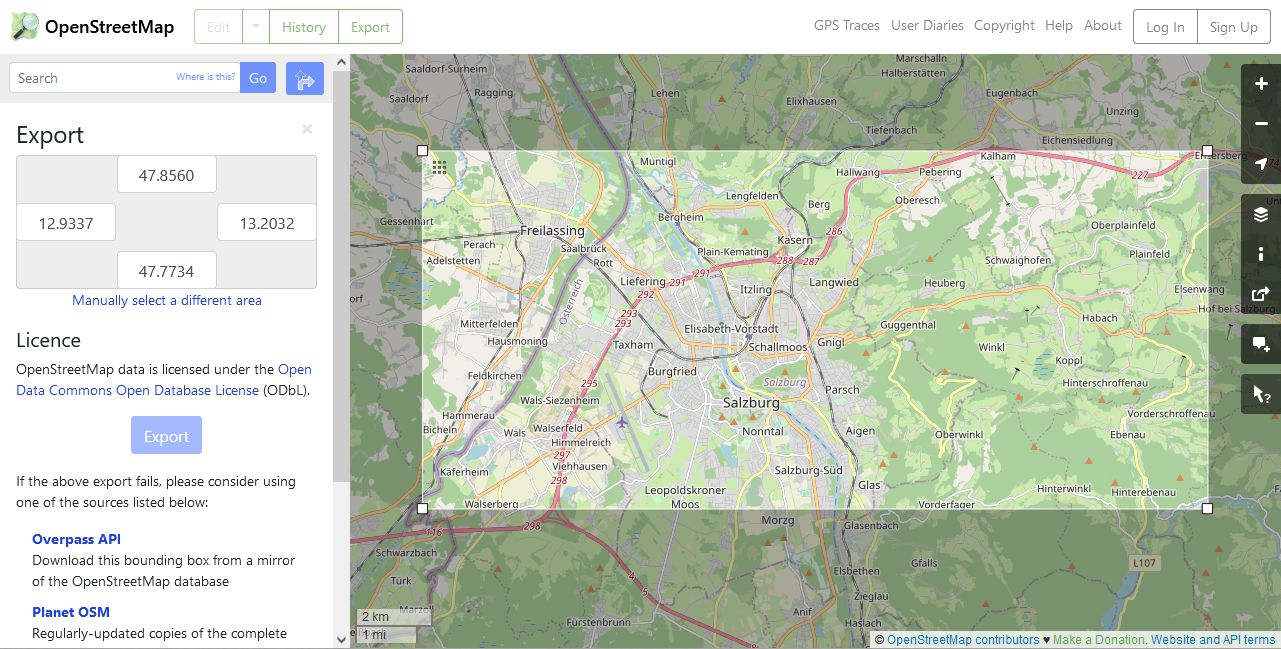
\includegraphics[width=0.9\textwidth]{images/BoundingBoxOSM.png}
  \caption{
  Bounding Box for extracted GPS trajectories.
  }
  %for reference to this figure
  \label{figure:BoundingBox}
\end{figure*}


\subsection{GPS Data}

%figure* stretches figure over both columns
\begin{figure*}[!ht]
  \centering
  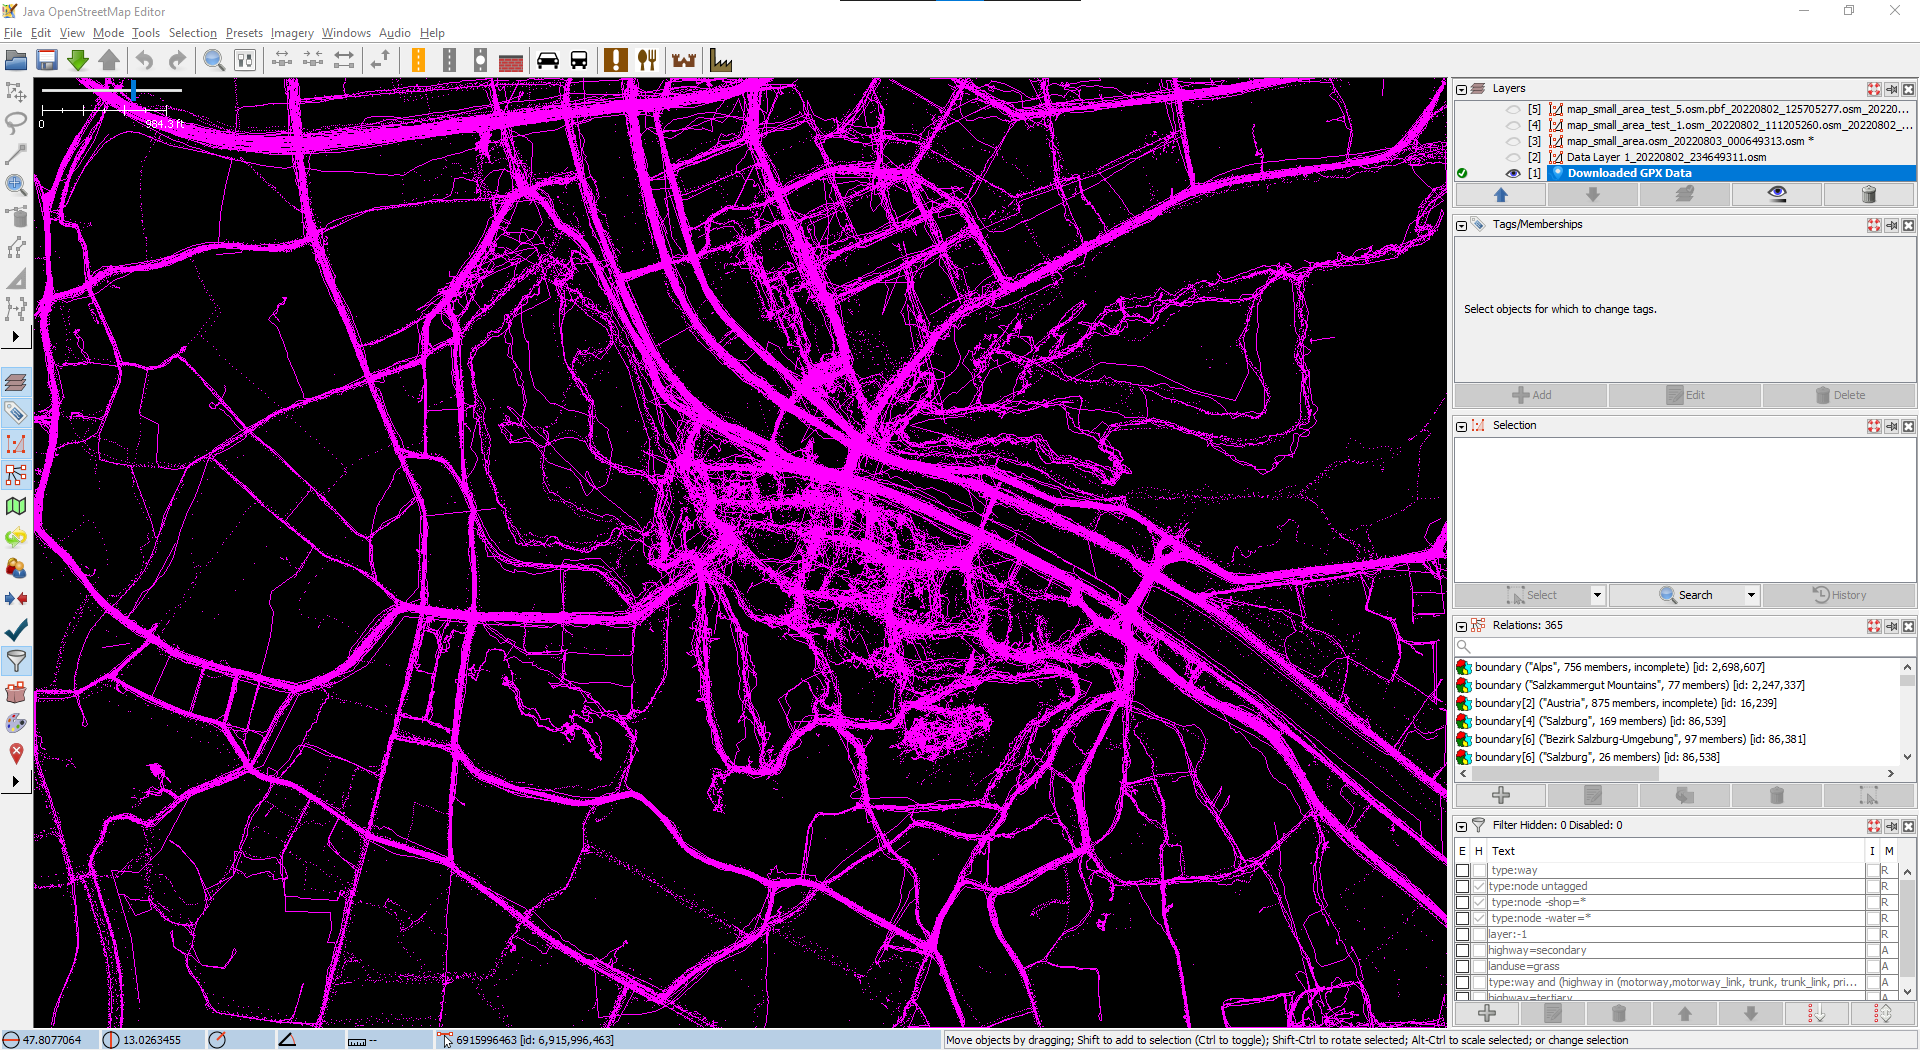
\includegraphics[width=0.7\textwidth]{images/GPSDataOSM.png}
  \caption{
  OSM GPS Data Overview.
  }
  %for reference to this figure
  \label{figure:MapData}
\end{figure*}

Given the bbox of Salzburg and its surroundings, 595.000 Data-points were extracted using the OSM Editing API. \footnote{\url{https://wiki.openstreetmap.org/wiki/API_v0.6#GPS_traces}}

\subsection{Map Data}

%figure* stretches figure over both columns
\begin{figure*}[!ht]
  \centering
  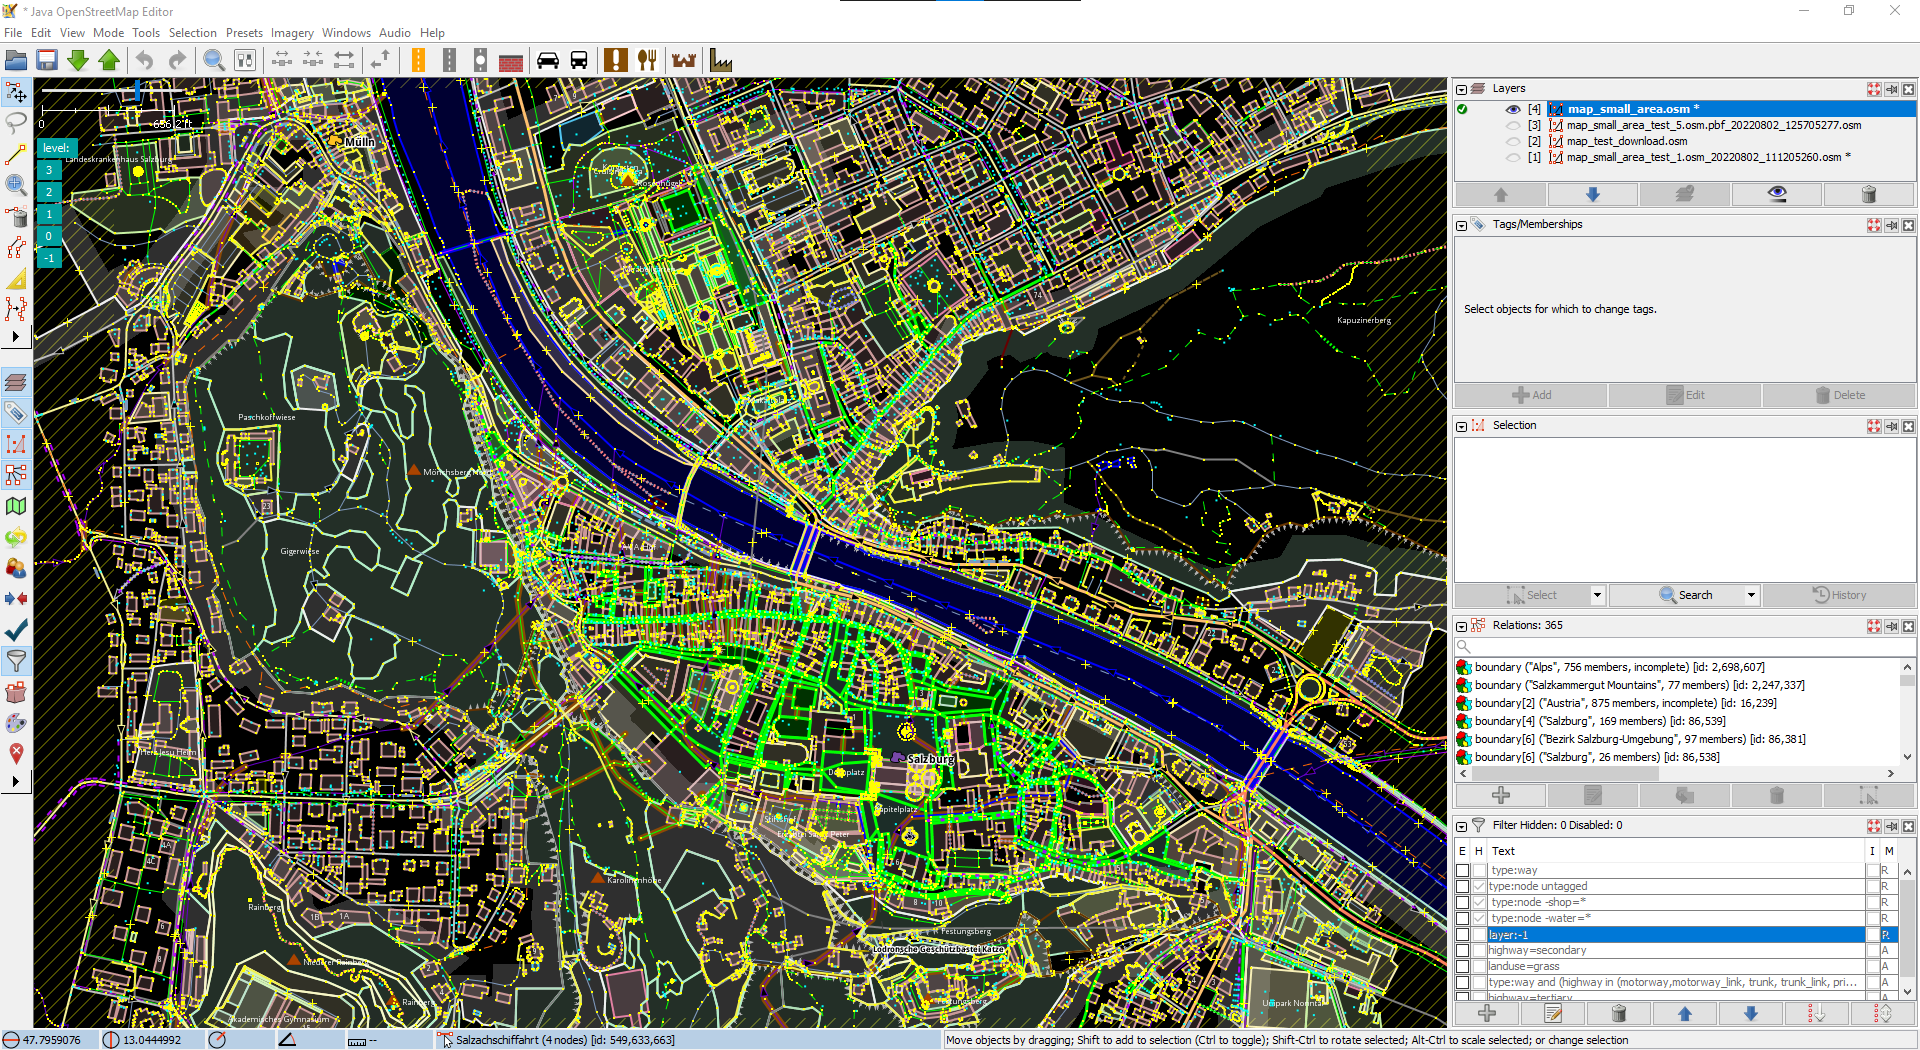
\includegraphics[width=0.7\textwidth]{images/DataOSM.png}
  \caption{
  OSM Map Data Overview.
  }
  %for reference to this figure
  \label{figure:MapData}
\end{figure*}

Same bbox

Consists of
- 28.158 nodes (2.929 incomplete)
- 19.427 ways (15.332 incomplete)
- 516 relations (197 incomplete)

- 333.831 nodes (7 incomplete)
- 43.604 ways (1.101 incomplete)
- 787 relations (422 incomplete)

%https://wiki.openstreetmap.org/wiki/JOSM_file_format
%https://wiki.openstreetmap.org/wiki/OSM_XML
%https://wiki.openstreetmap.org/wiki/PBF_Format

Further used for map-matching, geocoding & routing.


\section{Model & Implementation}

Provide implementation details such as the used software and our software architecture, highlight your own solutions to encountered difficulties. Describe relevant iterations of your implementation.

Before going deeper into the system architecture 
To go deeper into the system architecture 
Overview of the software basis used for the whole development: 
NodeJS, React,


Providing a route proposal starts further than analyzing geo-located trajectories. Precautious steps were needed in building the architecture to understand the data used for the newly suggested route. 

Therefore a Map Application was created to visualize the extracted and classified data, the routes used for the comparison, and the new suggested routes from the utilized routing engine. Said Map Application is a standalone React App using the Mapbox Plattform for map creation and route visualization. For working with React, Mapbox provides mapbox-gl-js, a javascript library that uses WebGL to render interactive maps from vector tiles and Mapbox styles.

%https://www.mapbox.com/
%https://docs.mapbox.com/mapbox-gl-js/guides/

For the map and route visualization to interact with the extracted geo trajectory data, a NodeJS backend was developed. The backend interacts with the OSM API and the established GeoDatabase, handling the trajectories' extraction, classification, and transformation.

With its geospatial data support, MongoDB was selected as the Geo-Database and stores the extracted Data-Set and the further classified data objects. Even though PostGIS is more mature and built on the Open Geospatial Consortium (OGC) standards, the uncertainty of incomplete data sets from the OSM project led to the decision to use the document-based solution.

To work with the OSM project and its map data, the JOSM was used to interact with the map layer as the basis for the route proposal. 
%https://josm.openstreetmap.de/

For the data extraction, a NodeJS backend interacting with the OSM API and the established GeoDatabase was created, handling the extraction, classification, and visualization of the trajectories and route suggestions.

Therefore a visualization of the City of Salzburg was built using the Mapbox Plattform. 
% https://docs.mapbox.com/mapbox-gl-js/guides/

% https://wiki.openstreetmap.org/wiki/Bounding_Box

\subsection{Database}

To work with NodeJS and MongoDB the decision was made to use Mongoose \footnote{\url{https://mongoosejs.com/}} as the object data modeling (ODM) or object relational mapping (ORM) library. \autocite[]{Mardan2014}

Mongoose enables a simple MongoDB database connection by defining the shape of the documents within a collection with a schema. Based on that schema models are compiled and the models are further responsible for creating and reading documents from the underlying MongoDB database.

The first collection schema in the database was modelled following the GeoJSON standard \footnote{\url{https://datatracker.ietf.org/doc/html/rfc7946}} and properties from the OSM GPS trajectory dataset. 

Properties mapped were "name", "description", "time", "url" and "coordTimes" while "coordTimes" being the timestamps for each coordinate given. 

For each processing step a new collection was created always having the initial OSM dataset for the bbox present for comparison and reversibility. 

Following schema have been created: 

\begin{itemize}
	\item TraceSchema
 	\item MapMatchedTraceSchema
 	\item GeoCodedMMTraceSchema
\end{itemize}

The TraceSchema was further extended after the pre-processing and classification to add the classification details:

\begin{lstlisting}
    classification: {
        avgSpeedSmallerThanNine: {
            type: Boolean
        },
        avgSpeedChunk100AverageSmallerThanNine: {
            type: Boolean
        }
    }
\end{lstlisting}



traceWaySchema

Collections created were 

Working with NodeJS and MongoDB the decision was made to use Mongoose as

Elegant MongoDB object modeling for Node.js


Working with MongoDB 

After the conversion the objects 
Working with Geodata there is 





MongoDB & Mongoose
% https://mongoosejs.com/docs/geojson.html
% https://www.mongodb.com/docs/manual/reference/geojson/

\subsection{Map Application}

\subsubsection{Frontend}

To work with GPS trajectories and map data a visualisation helps understanding about what that data means and how it is changing over the process steps taken. That was the reason leading to the decision to build a small Front-end Application (from here and further named \textit{Marshrut-Frontend}) that is able to make the data tangible and the process visible. The Marshrut-Frontend is built as a React Application.

The platform used to achieve that goal was Mapbox. As earlier mentioned in the System Overview Mapbox is a commercial map provider, yet they offer a lot of open-source tools and libraries and are mainly based on the OpenStreetMap Project.

Initially the whole Mapbox infrastructure was meant to be used for the entire research but due to limitation of free usage and not being able to customize map and street parameters without any efforts, only the map library for visualization was kept for the study.

The library used was the mapbox-gl-js library \footnote{\url{https://docs.mapbox.com/mapbox-gl-js/guides/}}. With the help of their javascript framework vector maps can be made interactive and using the Mapbox style specification \footnote{\url{https://docs.mapbox.com/mapbox-gl-js/style-spec/}}, it adds map styles to vector tiles that adhere to the Mapbox vector tile specification \footnote{\url{https://github.com/mapbox/vector-tile-spec}} and renders them using WebGL. 

%figure* stretches figure over both columns
\begin{figure*}[!ht]
  \centering
  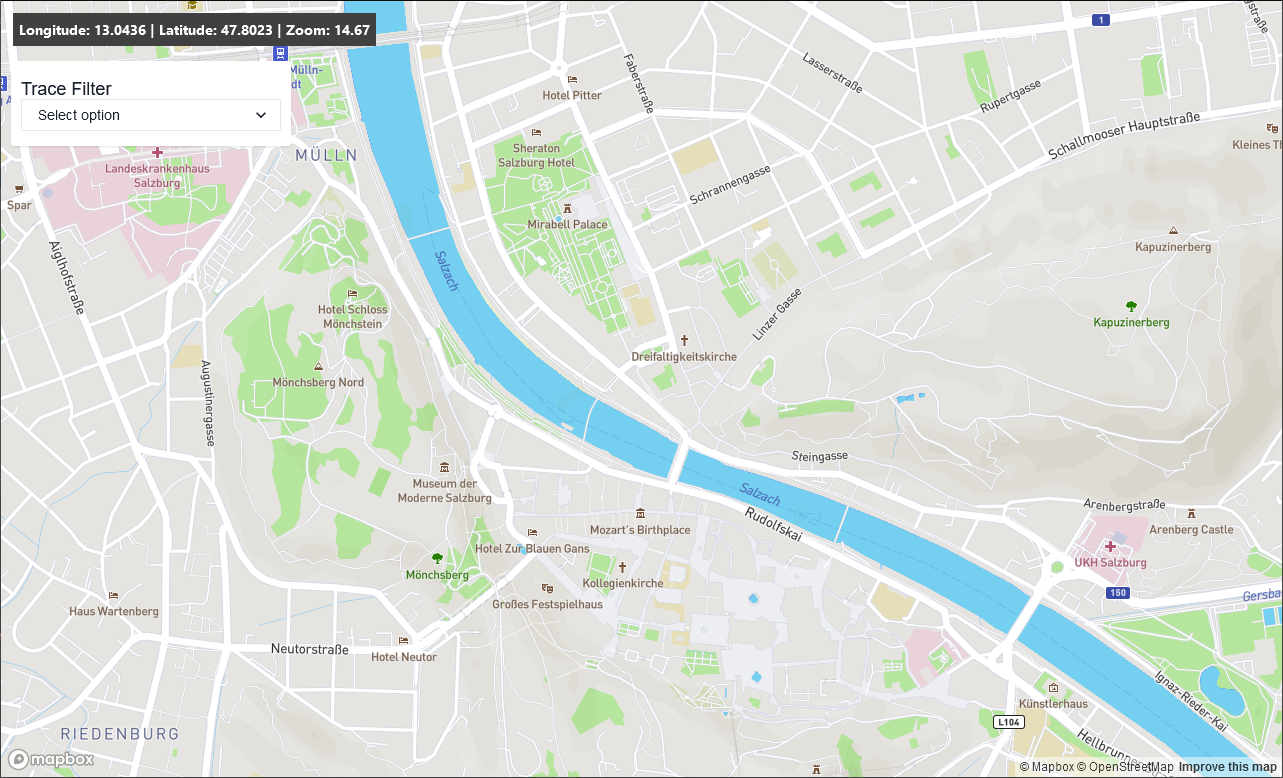
\includegraphics[width=0.9\textwidth]{images/MapApplicationWithout.png}
  \caption{
  Marshrut-Frontend
  }
  %for reference to this figure
  \label{figure:MarshrutFrontend}
\end{figure*}

To add the GPS trajectories the library is using a layering system. It enables to add vector, Raster DEM or GeoJSON sources. To display the trajectories used in the research the GeoJSON source option was selected as further described the traces extracted from the OSM data-set will be using that exact format. 

%figure* stretches figure over both columns
\begin{figure*}[!ht]
  \centering
  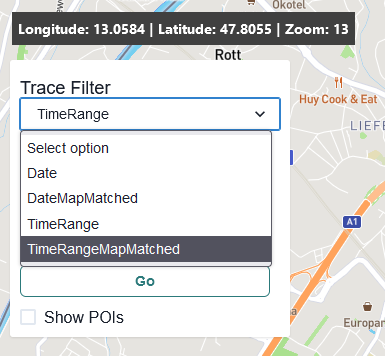
\includegraphics[width=0.4\textwidth]{images/MapApplicationFilterOptions.png}
  \caption{
  Marshrut-Frontend Filter Options
  }
  %for reference to this figure
  \label{figure:FilterOptions}
\end{figure*}

The visualization of the different phases was the main goal of creating the Map Application. To be able to filter the layer output and switch between the steps the Trace Filter menu as seen in \ref{figure:FilterOptions} was added. With the filter a selection of trace by date and traces by time-range was made possible per each step. Steps visualized were unclassified / raw and classified & map-matched. 

As working with GPS trajectories and map data without a visualisation is 

\subsubsection{Backend}

To handle the data coming from the API, database and Marshrut Front-end a Back-end (from here and further named \textit{Marshrut Back-end}) was developed. Written in NodeJS its purposes are to do the data extraction, process the data through all processing steps, act as the database connector for the Marshrut Front-end and serve as the API layer for the map adaption & routing customization.

\subsection{Data Extraction}

Using the OSM Editing API the GPS trajectories were extracted according to the API documentation. \footnote{\url{https://wiki.openstreetmap.org/wiki/API_v0.6#GPS_traces}} The API Results were then each saved as .gpx files to be then ready for the Data Conversion step. In total 119 files containing each 5000 data points were extracted for the boundary box used for the research.


% https://www.topografix.com/GPX/1/1/#type_trksegType

\begin{lstlisting}
<?xml version="1.0" encoding="UTF-8"?>
<gpx version="1.0" creator="OpenStreetMap.org" xmlns="http://www.topografix.com/GPX/1/0">
    <trk>
        <name>osmtrack_KUnrl0ZaKm.gpx</name>
        <desc>desc.</desc>
        <url>/user/exbrick/traces/3444105</url>
        <trkseg>
            <trkpt lat="47.8318200" lon="13.0567170">
                <time>2006-08-22T01:37:05Z</time>
            </trkpt>
            <trkpt lat="47.8325810" lon="13.0567800">
                <time>2006-08-22T01:37:20Z</time>
            </trkpt>
            <trkpt lat="47.8331180" lon="13.0569120">
                <time>2006-08-22T01:37:30Z</time>
            </trkpt>
            
\end{lstlisting}

\subsection{Data Prepocessing}

\subsubsection{Conversion}

As the objects returned from the API are in the GPX Format, a conversion step was needed to further work with the trajectories. As the MongoDB Database and the libraries used in the built Map Application are working with the GeoJSON standard \footnote{\url{https://datatracker.ietf.org/doc/html/rfc7946}}, a conversion step was necessary.

The conversion was achieved using the open-source "toGeoJSON" tool \footnote{\url{https://github.com/mapbox/togeojson}} provided by Mapbox. After the first objects were converted, a significant number of them had property attributes missing after the conversion. Therefore, the tool was adapted according to the GPX Formats given attributes used by the OSM Editing API.

The property attributes used by the OSM Editing API are the following:

\begin{itemize}
	\item name
	
	Name of the uploaded Route
	
 	\item desc
 	
 	User Description
 	
 	\item time
 	
 	Upload Time
 	
 	\item url
 	
 	URL to OSM Database
 	
 	\item coordTimes
 	
 	Array of Timestamps
 	
\end{itemize}

The "url"-property was the one that has been missing and was added adapting the node package. Even-though the "url"-property property was not necessarily needed for the next processing steps it was still kept for consistency validation of the traces.

Converting the 595.000 data-points resulted in 533 routes to be further used.


% Attributes added: Properties

% Using the tool togeojson provided by Mapbox the conversion was 

% https://github.com/mapbox/togeojson

\subsubsection{Outlier Removal}



\subsection{Map-Matching}

Cleaning up and matching the traces to the paths and streets they have supposedly been recorded on a map-matching algorithm had to be used. For this purpose the Mapbox Map Matching API \footnote{\url{https://docs.mapbox.com/api/navigation/map-matching/}} was initially intended to be used. On the further tool and software selection process yet the OSRM routing engine was selected to fit for as the router of the research. As the OSRM Project comes with its own Map Matching service \footnote{\url{http://project-osrm.org/docs/v5.24.0/api/#match-service}} a comparison of both the accuracy's and outcomes was obvious and necessary.

Consequently a local instance of the OSRM Project was needed to be established as their demo has no public endpoint available to be used. To speedup the local setup a docker image provided by the project was setup and selected as the way to go. Before that checking out the whole project and performing an analysis on possibly needed customization was done, yet as the docker instance was also able to be adapted in the ways needed, this path was not longer considered.

To setup the docker image their setup guide \footnote{\url{https://hub.docker.com/r/osrm/osrm-backend/}} was followed accordingly.

To compare both the OSRM Match service and the Mapbox Map Matching API tests were completed using the same non-matched route against the two algorithms. Selection criteria was on the one hand a visual examination of both matching results using the Marshrut Front-end and on the other hand the error rate of how many points were not being able to be matched by the algorithm of either. 

Both services were called with the help of the Marshrut Back-end and the results then visualized as seen in \ref{} and \ref{}:  

Image of Map-Match result OSRM

Image of Map-Match result Mapbox

\subsubsection{OSRM}

\subsubsection{Mapbox}

Result of the comparison was that the Mapbox Map Matching API was visually and error rate wise better performing than the OSRM Match service. That was the reason why the Map-Matching was performed using the Mapbox API to get more accurate pedestrian traffic patterns for the routing engine. 

All of the 533 converted routes were then sent to the Mapbox API and after matching saved in Database using the MapMatchedTrace Model established earlier. 

The MapMatchedTraceSchema is an iteration of the TraceSchema, yet the geometric fields stayed the same and were just replaced by the map-matched coordinates to not violate the GeoJSON standard so the traces can be visualized the same as the non-matched one in the Marshrut Front-end.


\autocite[]{Delling2012}

\subsection{Data Classification}

The Data Classification

However, GPS traces are stored in plain text formats with no attached metadata such as, transportation mode, length, or speed. This not only makes managing large volumes of GPS traces inefficient but also restricts the scale and scope of algorithms for human mobility pattern detection

Road networks are built upon GPS traces uploaded by registered users and can be edited or updated manually at any time. A description can be associated to a GPS trace while being uploaded but there are no additional required metadata or restrictions

 This means the transportation mode of the GPS trace (e.g. walking, motoring, or boating) cannot be known in the database which in turn limits the data- base’s applications. Besides, they do not store additional metadata, such as average speed or total length of the GPS trace which can be automatically calculated. Such metadata not only facilitates analyzing, mining, and visualizing large volumes of GPS traces, but also paves the path for automatic applications of GPS traces.


\autocite[]{Zhang2012}

As the OSM GPS Traces are randomized and 

Count 533

3 Layers




Finding Routes Name / Description Car / Auto

NameCnt: 76
DescCnt: 8
Count: 397

Avg speed on total route

Avg speed using segmentation




TurfJS


osrm

Mapbox API


%However, GPS traces are stored in plain text formats with no attached metadata such as, transportation mode, length, or speed. This not only makes managing large volumes of GPS traces inefficient but also restricts the scale and scope of algorithms for human mobility pattern detection. Open Street Map (OSM), founded in UK in 2004 with more than 1 million registered users (Wood, 2013), is the most prominent volunteered geographic information devoted to providing a free map of the world emphasizing the road networks. Road networks are built upon GPS traces uploaded by registered users and can be edited or updated manually at any time. A description can be associated to a GPS trace while being uploaded but there are no additional required metadata or restrictions (https://www.open- streetmap.org/traces; OpenStreetMap, n.d.). This means the transportation mode of the GPS trace (e.g. walking, motoring, or boating) cannot be known in the database which in turn limits the data- base’s applications. Besides, they do not store additional metadata, such as average speed or total length of the GPS trace which can be automatically calculated. Such metadata not only facilitates analyzing, mining, and visualizing large volumes of GPS traces, but also paves the path for automatic applications of GPS traces. Examples of such applications are automatic road and pedestrian network construction (Hashemi, 2017b), recognizing POIs (Bhattacharya, Kulik, & Bailey, 2015), developing intelligent location-based services (Liu & Karimi, 2006), detecting individual (Song et al., 2010), or collective (Becker et al., 2013; Harder, Nes, Jensen, Reinau, & Weber, 2012) mobility patterns, and real-time event detection which is of great value to municipalities, police, and fire departments.



\subsection{Reverse Geo-coding}

For having now all routes sorted out and only classified routes available to build the historic pedestrian traffic patterns, the streets and paths taken have to be found and counted to then be transferred onto the map used for the routing engine. 

Therefore the reverse geo-coding method was set-in to find the correlating map information to the GPS points of the traces. To achieve that the Nominatim Geo-coder was chosen to be the solution to achieve the goal. Number one reason to use the solution from the Nominatim project was that the project is based on the OSM data and is so able to result back in not only map information but to result in OSM data IDs to specific ways the GPS points are laying on. 

The Nominatim project offers a public API service to use each their Geo-coding and Reverse Geo-coding service. Still the public API comes with a Usage Policy (named by them-self the Geo-coding Policy) not allowing heavy use meaning bulk Geo-coding of larger amounts is not encouraged. This is the reason for setting it up locally do not have to comply with their Geo-coding Policy. To do so, following their local installation instructions \footnote{\url{https://nominatim.org/release-docs/latest/admin/Installation/}}, another docker instance was setup for the researches purposes. This was done by using their docker repository \footnote{\url{https://github.com/mediagis/nominatim-docker}} as it was the easiest and least complex way to get the services running locally.

Having the Nominatim project running, all 397 routes remaining after the classification phase were reverse Geo-coded. Each GPS Location of each route was sent to the reverse Geo-coding service and then saved in the Database using the GeocodedMMTrace Model established earlier. 

The GeocodedMMTraceSchema was again an iteration of the original TraceSchema adding an array of objects named geoCoding to the original structure. The array contains each coordinate and the geoCoding 




\subsection{Map Adaptations}

JOSM




\subsection{Routing}

Routing Engine

Profile adaption

\begin{lstlisting}
        smoothness_speeds = {
            excellent = walking_speed,
            bad = walking_speed * 0.5,

            one = walking_speed*0.01,
            two = walking_speed*0.02,

            three = walking_speed*0.001,
            four = walking_speed*0.004,
            
            five = walking_speed*0.005,
            six = walking_speed*0.006,
        }
\end{lstlisting}

\autocite[]{Delling2012}


\section{Evaluation}
%Describe your methodology. How did you evaluate your work? Why did you choose this methodology? Present results of your evaluation here.

To evaluate the research and to measure a possible increase in satisfaction of the route proposal a trail run of two routes with equal starting and ending point was conducted. Starting point of the routes was the Mozart Square near the cathedral and ending point was the Mirabell gardens. Both points were selected as they are touristic points of interests and usually the spots and the routes are visited and used by a lot of people during the year. Also due to the street network of Salzburgs limited alternatives a route directly in the hearth of the city was preferred. This was a strategic decision as also locals who were taking part in the trial are mostly using standard routes to get there and so the effect of the bias of already knowing the city and city routes will be minimized.

The route to compare the new proposed route to was the first and fastest route suggested by the routing functionality from Google Maps. 

\subsection{Methodology}

A qualitative trail run was conducted to measure a possible increase in satisfaction with the route proposal. In the trial run, the standard route was compared to the newly proposed route and measured using one survey. 

The survey was structured in three parts. Part number one used a quantitative method to determine the subjects demographics and general walking and route choosing behavior. Part number two measures the satisfaction of both routes. And part number three compares the routes within each other.

Finding out about the subjects' general walking and route choosing behavior should give a better understanding of the route satisfaction part results. Furthermore, it will give a relation to the increase or decrease in satisfaction.


% Survey number one uses a quantitative method to determine the subjects' general travel behavior, while survey number two compares and measures satisfaction with a quantitative approach after the trial run.



% Quantitative Surveys.




% In present work, various research methods have been applied. They include a descriptive method (outlining different approaches to the term "actorness" and identifying the ways of measuring it), a historical method (following the historical development of the shared energy and environmental policies in the EU and their adaptation to the realities of the modern world), a comparative method (e.g., conferring the definitions of actorness and the level of actorness of the EU in energy and environmental spheres), statistical and quantitative (e.g., providing statistical data on the ecological goals and sustainable development, import of energy resources), analytical (e.g., assuming how the public opinion on the ecological situation contributes to the changing of the adopted energy policies), and process tracing method (e.g., identifying the causal mechanisms that link opportunity, presence, capability, performance, and effect, i.e., EU actorness).




\subsection{Survey}

The survey was developed with the influence of general pedestrian, walking and satisfaction surveys. (Sources) It is split into three parts evaluated separately, yet presented to the trial participants as one document that was filled out on the course of taking the routes. Part one containing the demographics, general walking behavior and route choosing behavior chapters were filled out before taking the first route to have time to explain the survey setup and to get the first details about the person taking the routes. Part two consisting the evaluation of the routes taken was filled out each time after reaching the goal of the trips. And part three, the comparison, was done after the trial run to find out how each participant felt after taking both routes.

As route choosing is depending on multiple factors (environmental, personal, ...)


Part one should get a better knowledge about the persons demographics. 


PEDESTRIAN SURVEY

\subsection{Survey Questions}
\newcounter{surveyCounter}

\subsubsection{Demographics}

\begin{enumerate}
    \item What is your age?
    \begin{itemize}
        \item 0-15 years
        \item 15-30 years
        \item 30-45 years
        \item 45+
        \item Prefer not to say
    \end{itemize}
    
    \item What gender do you feel you belong?
    \begin{itemize}
        \item Female
        \item Male
        \item Prefer not to say
    \end{itemize}
    
    \item What is your highest educational qualification?
    \begin{itemize}
        \item No compulsory education 
        \item Compulsory school or secondary school (polytechnic school)
        \item Apprenticeship 
        \item Vocational middle school without Matura (e.g., 3-year HBLA/HLWM) 
        \item General education or vocational higher school with Matura (e.g., Gymnasium, HTL, HAK, HLWM, HBLA) 
        \item Bachelor's Degree
        \item Master's Degree
        \item Ph.D. or higher
        \item Prefer not to say
    \end{itemize}
    
    \item What would you describe the area you’re living in as?
    \begin{itemize}
        \item Urban
        \item Rural
    \end{itemize}
    
    \item How long have you been living in Salzburg?
    \begin{itemize}
        \item ~1 year
        \item 1-5 years
        \item 5-10 years
        \item 10+ years
    \end{itemize}
    
    \item Do you drive a car?
    \begin{itemize}
        \item Yes
        \item No
    \end{itemize}
    \setcounter{surveyCounter}{\value{enumi}}
\end{enumerate}


\subsubsection{General Walking Behavior}

\begin{enumerate}
    \setcounter{enumi}{\value{surveyCounter}}
    
    \item What are the purposes of your walk trips in general? (Choose a few)
    \begin{itemize}
        \item Exercise/outdoor recreation
        \item Grocery/food shopping
        \item Personal business
        \item Medical appointment
        \item Entertainment
        \item Dining at restaurants or bars
        \item Commute to work
        \item Other work-related travel
        \item Other
        \item No walking
    \end{itemize}
    
    \item How frequent do you take walking trips per month?
    \begin{itemize}
        \item 1 to 2 trips
        \item 3 to 6 trips
        \item 7 to 10 trips
        \item 11 to 19 trips
        \item 20 trips or more
    \end{itemize}
    
    \item How long are your walking trips in general?
    \begin{itemize}
        \item 5 to 10 minutes
        \item 10 to 20 minutes
        \item 20 to 40 minutes
        \item 40 to 60 minutes
        \item Greater than 60
    \end{itemize}
    
    \item Do you take walk trips on vacation?
    \begin{itemize}
        \item Yes
        \item No
    \end{itemize}
    
    \setcounter{surveyCounter}{\value{enumi}}
\end{enumerate}

\subsubsection{Route Choosing Behavior}

\begin{enumerate}
    \setcounter{enumi}{\value{surveyCounter}}
    
    \item How do you plan your route?
    \begin{itemize}
        \item Physical map
        \item Map Application (Google Maps, …)
        \item Tour guide
        \item Other, please specify: __________________
    \end{itemize}
    
    \item When do you plan your route?
    \begin{itemize}
        \item Before the trip
        \item On the spot
    \end{itemize}
    
    \item What are the main factors for your route planning? (Choose up to 3)
    \begin{itemize}
        \item Travel Time
        \item Distance
        \item Least directional changes
        \item Road Condition
        \item Crowdedness
        \item Many attractive places
        \item Weather
    \end{itemize}
    
    \item When you are on vacation does your route planning change?
    \begin{itemize}
        \item Yes
        \item No
    \end{itemize}
    
    \item If yes, what factors do change?
    \begin{itemize}
        \item Travel Time
        \item Distance
        \item Least directional changes
        \item Road Condition
        \item Crowdedness
        \item Many attractive places
        \item Weather
    \end{itemize}
    
    \setcounter{surveyCounter}{\value{enumi}}
\end{enumerate}

\subsubsection{Route A}

\begin{enumerate}
    \setcounter{enumi}{\value{surveyCounter}}
    
    \item How was the travel time on the route? 
    \begin{itemize}
        \item Unsatisfying
        \item Satisfying
    \end{itemize}
    
    \item How crowded was the route?
    \begin{itemize}
        \item Deserted
        \item Very Crowded
    \end{itemize}
    
    \item How much you were satisfied by the route overall? 
    \begin{itemize}
        \item Very unsatisfied
        \item Very satisfied
    \end{itemize}
    
    \item What were the factors leading to this level of satisfaction?
    \begin{itemize}
        \item Travel Time
        \item Distance
        \item Least directional changes
        \item Road Condition
        \item Crowdedness
        \item Many attractive places
        \item Weather
    \end{itemize}
    
    
    \setcounter{surveyCounter}{\value{enumi}}
\end{enumerate}

\subsubsection{Route B}

\begin{enumerate}
    \setcounter{enumi}{\value{surveyCounter}}
    
    \item How was the travel time on the route? 
    \begin{itemize}
        \item Unsatisfying
        \item Satisfying
    \end{itemize}
    
    \item How crowded was the route?
    \begin{itemize}
        \item Deserted
        \item Very Crowded
    \end{itemize}
    
    \item How much you were satisfied by the route overall? 
    \begin{itemize}
        \item Very unsatisfied
        \item Very satisfied
    \end{itemize}
    
    \item What were the factors leading to this level of satisfaction?
    \begin{itemize}
        \item Travel Time
        \item Distance
        \item Least directional changes
        \item Road Condition
        \item Crowdedness
        \item Many attractive places
        \item Weather
    \end{itemize}
    
    
    \setcounter{surveyCounter}{\value{enumi}}
\end{enumerate}

\subsubsection{Route Comparison}

\begin{enumerate}
    \setcounter{enumi}{\value{surveyCounter}}
    
    \item Which of the two routes satisfied you more?
    \begin{itemize}
        \item Route A
        \item Route B
    \end{itemize}
    
    \item Which of the two routes was less crowded?
    \begin{itemize}
        \item Route A
        \item Route B
    \end{itemize}
    
    \item Would you take one of the routes if not given?
    \begin{itemize}
        \item  Yes
        \item No
    \end{itemize}
    
    \item If yes, which one?
    \begin{itemize}
        \item Route A
        \item Route B
    \end{itemize}
    
    \setcounter{surveyCounter}{\value{enumi}}
\end{enumerate}



Part 1
Part 2
Part 3

\subsection{Trial run}

The trial run was executed with 20 people in the span of four days. Each round was taken individually with every participant. Per day runs were done during different times of the day reaching from 09:00 to 18:00. To minimize the redundant walking time to get back to the starting point the routes were taken once from Mozartplatz to Mirabellgarden and then from Mirabellgarden to Mozartplatz. This decision was made as finding participants was already not easy so taking the round trip instead of starting at the same spot saved time for both parties. And the factor of crowdedness is not going to be affected no matter the direction. 

\subsubsection{Day one}

\begin{itemize}
    \item Day: Friday 
    \item Date: 29th of July
    \item Weather: Partly sunny
    \item Temperature: 20 - 28 degrees Celsius
    \item Humidity: 40 - 73 percent
    \item Participants: 2
\end{itemize}

\subsubsection{Day two}

\begin{itemize}
    \item Day: Saturday 
    \item Date: 30th of July
    \item Weather: Partly sunny
    \item Temperature: 17 - 23 degrees Celsius
    \item Humidity: 51 - 93 percent
    \item Participants: 3
\end{itemize}

\subsubsection{Day three}

\begin{itemize}
    \item Day: Sunday 
    \item Date: 31th of July
    \item Weather: Overcast
    \item Temperature: 19-26 degrees Celsius
    \item Humidity: 40 - 77 percent
    \item Participants: 10
\end{itemize}

\subsubsection{Day four}

\begin{itemize}
    \item Day: Monday 
    \item Date: 1st of August
    \item Weather: Partly sunny
    \item Temperature: 22 - 28 degrees Celsius
    \item Humidity: 40 - 77 percent
    \item Participants: 4
\end{itemize}

\subsection{Results}

%figure* stretches figure over both columns
\begin{figure*}[!ht]
  \centering
  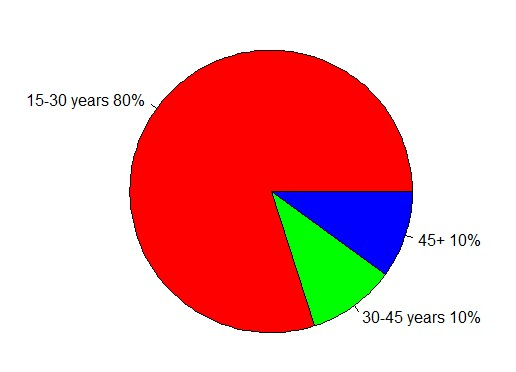
\includegraphics[width=0.4\textwidth]{images/AgeDistributionNew.jpg}
  \caption{
  Gender Distribution.
  }
  %for reference to this figure
  \label{figure:GenderDistribution}
\end{figure*}

%figure* stretches figure over both columns
\begin{figure*}[!ht]
  \centering
  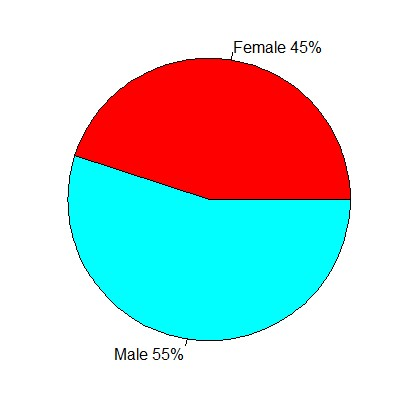
\includegraphics[width=0.3\textwidth]{images/GenderDistributionNew.jpg}
  \caption{
  Gender Distribution.
  }
  %for reference to this figure
  \label{figure:GenderDistribution}
\end{figure*}

%figure* stretches figure over both columns
\begin{figure*}[!ht]
  \centering
  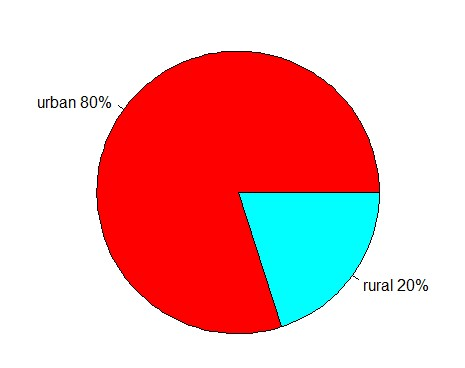
\includegraphics[width=0.3\textwidth]{images/LivingAreaDistribution.jpg}
  \caption{
  Gender Distribution.
  }
  %for reference to this figure
  \label{figure:GenderDistribution}
\end{figure*}

%figure* stretches figure over both columns
\begin{figure*}[!ht]
  \centering
  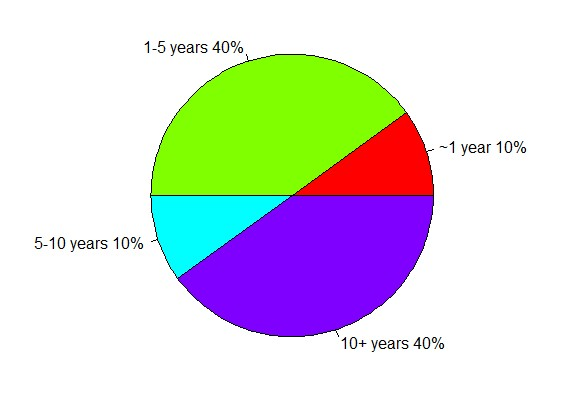
\includegraphics[width=0.4\textwidth]{images/LivingTimeDistribution.jpg}
  \caption{
  Gender Distribution.
  }
  %for reference to this figure
  \label{figure:GenderDistribution}
\end{figure*}

Traveltime

> t1 <- c(4,4,5,5,5,4,5,5,4,5,5,4,4,5,5,4,3,3,3,5)
> t2 <- c(5,4,5,5,5,5,4,5,4,4,3,3,4,3,5,4,4,4,4,5)
> wilcox.test(t1, t2, paired = TRUE, alternative = "greater")

	Wilcoxon signed rank test with continuity correction

data:  t1 and t2
V = 32.5, p-value = 0.3134
alternative hypothesis: true location shift is greater than 0


Crowdeness

> c1 <- c(5,3,5,3,2,3,3,4,4,3,2,4,5,4,5,4,4,4,5,3)
> c2 <- c(1,2,2,1,1,1,2,2,2,1,1,1,2,1,2,2,1,2,2,1)
> wilcox.test(c1, c2, paired = TRUE, alternative = "greater")

	Wilcoxon signed rank test with continuity correction

data:  c1 and c2
V = 210, p-value = 3.855e-05
alternative hypothesis: true location shift is greater than 0


Satisfaction

> x <- c(3,4,4,5,5,4,4,4,4,5,5,3,4,4,5,4,3,4,3,5)
> y <- c(5,5,5,5,5,4,4,5,4,4,3,3,5,4,5,4,4,4,4,5)
> wilcox.test(x, y, paired = TRUE, alternative = "greater")

	Wilcoxon signed rank test with continuity correction

data:  x and y
V = 12.5, p-value = 0.9051
alternative hypothesis: true location shift is greater than 0



\section{Discussion}
Discuss your results to answer your research question. Does your data support you hypotheses? Put your results into perspective by situating it in the research field/related work.

\section{Conclusion and Future Work}
Summarize your work, outline limitations and future work. 

% \section{Formatierung}
% \label{section:Formatting}

% Text mit beliebigen Sonderzeichen in UTF-8 ohne BOM \ldots
% ,
% \textbf{hervorgehobener Text},
% \texttt{void}\footnote{Fußnote 1},
% mathematische Formel im Text $\sum_{i=0}^n i^2$
% \ldots

% Referenz auf Unterabschnitt \ref{subsection:Coding} der Arbeit, automatisch richtig nummeriert.

% \textcite[]{Mulloni:2010} für einen einen Literaturverweis im laufenden Text.

% Literaturverweise sind essentiell für eine wissenschafliche Arbeit. \autocite[]{McConnell:2004:CCS:1096143}.

% Achtung: nur zitierte Literatur wird im Literaturverzeichnis
% angeführt.\footnote{Fußnote 2}


% Wir verwenden \LaTeX\footnote{ \url{http://en.wikibooks.org/wiki/LaTeX}} -- und das
% ist keine Quelle, sondern blos eine URL.

% \subsection{Figures machen was sie wollen}

% % h = try to place the figure Here
% % t = try to place the figure at the Top of a page
% % p = try to place this figure along with others on a separate Page
% % Note that LaTeX has a sophisticated ranking algorithm to place figures.
% % It is not always easy to accept LaTeX's placing but it is harder doing it
% % manually. Just let it go ;-)
% \begin{figure}[!ht]
% 	\centering
% 	\subfloat[Das Julia Fraktal]{
% 		\includegraphics[width=0.75\linewidth]{images/Julia-Fractal.png}
% 		%for reference of this subfigure only
% 		\label{subfigure:Julia-Fractal}
% 	}
% 	\qquad
% 	\subfloat[Noise für Tinteneffekte]{
% 		\includegraphics[width=0.75\linewidth]{images/Perlin-Coherent.png}
% 		%for reference of this subfigure only
% 		\label{subfigure:Perlin-Coherent}
% 	}
% 	\caption[
% 		Verschiedene Pixelgraphiken\newline
% 		% source url given in the table of figures
% 		\small\texttt{https://mediacube.at/wiki/}
% 	]{
% 		Verschiedene Pixelgraphiken
% 	}
% 	%for reference to all subfigures
% 	\label{figure:PixelImages}
% \end{figure}

% Unterstützte Pixelgraphikformate: PNG, JPEG, PDF.
% Angabe von height oder width meist wichtig.

% Referenz auf Abbildung \ref{figure:PixelImages} mit allen Teilbildern.
% Referenz auf Unterabbildung \ref{subfigure:Julia-Fractal}.

% %figure* stretches figure over both columns
% \begin{figure*}[t]
% 	\centering
% 	\includegraphics[width=0.9\textwidth]{images/KappaGamma.pdf}
% 	\caption{
% 		Vektorgraphik mit \LaTeX\ Beschriftung ($\kappa$, $\gamma$)
% 	}
% 	%for reference to this figure
% 	\label{figure:KappaGammaTau}
% \end{figure*}

% Referenz auf Abbildung \ref{figure:KappaGammaTau}.

% Bei Vektorgraphik mit \LaTeX\ Beschriftung keine Skalierung mit width oder height verwenden.

% Vektorgraphik mit \LaTeX\ Beschriftung kann etwa mit \texttt{ipe} erstellt werden.

% Unterstütztes Vektorgraphikformat: PDF. EPS muss konvertiert werden.


% \subsection{Unterabschnitt 2}
% %for references to this subsection
% \label{subsection:Coding}

% \begin{lstlisting}[
% 	label=listing:Main, %for reference to this listing
% 	float=h,
% 	caption=main.cpp,
% 	firstnumber=10
% ]
% int main(void) {
% 	while (true) {
% 	}
% 	return 0;
% }
% \end{lstlisting}

% Wie man in Listing \ref{listing:Main} in Zeile 10 sieht, kann man die Zeilennummern im Listing absichtlich setzen, hier z.B. auf 10. In Listing \ref{listing:closure} wurde davon nicht Gebrauch gemacht. In diesem Fall beginnt die Nummerierung bei 1.

% \begin{lstlisting}[
%     label=listing:closure,
% 	float=h,
% 	caption=Closure in Javascript,
% 	language=JavaScript
% ]
% function foo(x,y) {
%     let i = x;
%     return function(a) {
%         return i * 2;
%     }
% }
% \end{lstlisting}


% \subsubsection{Unterunterabschnitt i}

% Wörtliches Zitat:
% %select proper language if not in German
% \selectlanguage{english}
% \begin{quote}
% ``Erwin Unruh discovered that templates can be used to compute
% something at compile time. [...] The intriguing part of this exercise, however, was that the production of the prime numbers was performed by the compiler during the compilation process and not at run time.''

% \autocite[305]{Bosch2014}
% \end{quote}
% %select German again or the language that you were using before (note ngerman stands for New German)
% %\selectlanguage{ngerman}
% \selectthesislanguage


% \subsection{Unterabschnitt b}

% \begin{enumerate}
% 	\item Punkt 1
% 	\begin{enumerate}
% 		\item Unterpunkt 1
% 		\item Unterpunkt 2
% 	\end{enumerate}
% 	\item Punkt 2
% \end{enumerate}

% \begin{itemize}
% 	\item Punkt 1
% 	\begin{itemize}
% 		\item Unterpunkt 1
% 		\item Unterpunkt 2
% 	\end{itemize}
% 	\item Punkt 2
% \end{itemize}


% \subsection{Unterabschnitt c}

% \begin{table}[ht]
% 	\centering
% 	\begin{tabular}{r|rrr}
% 		    & $i$ & $j$ & $k$ \\ \hline
% 		$i$ &$-1$ & $k$ &$-j$ \\
% 		$j$ &$-k$ &$-1$ & $i$ \\
% 		$k$ & $j$ &$-i$ &$-1$
% 	\end{tabular}
% 	\caption{
% 		Multiplikationstabelle für Quaternionen
% 	}
% 	\label{table:Quaternions}
% \end{table}

% Referenz auf Tabelle \ref{table:Quaternions}.

% \section{Abschnitt 2}
% \label{section:MathematicalStuff}

% Sei $f(x)$ eine stetige Funktion, so ist die \textbf{Fourier Transformierte}
% $F(\omega)$ wie folgt definiert:
% \begin{equation}
% \label{equation:FourierDefinition}
% 	F(\omega) = \int_{-\infty}^{\infty} f(x) e^{-i\omega t} dt
% \end{equation}

% Referenz auf mathematische Gleichung (\ref{equation:FourierDefinition}).

% Unnummerierte Gleichung:
% \begin{equation*}
% 	e^{i\varphi} = \cos\varphi + i \sin\varphi
% \end{equation*}
% %you may also use \[ \] instead of \begin{equation*} and \end{equation*}

% Gleichungssystem:
% \begin{eqnarray}
% 	g(x) = f(x - x_0) & \Leftrightarrow &
% 		G(\omega) = F(\omega) e^{-i\omega x_0} \\
% 	g(x) = f(x) e^{i\omega_0 x} & \Leftrightarrow &
% 		G(\omega) = F(\omega - \omega_0)
% \end{eqnarray}
